\section{Approach}

Implementing Tweether has multiple steps which are composed of individual and interconnected components. We use both the weather data and the Twitter data in our study (Section~\ref{sec:dataset}). Based on the clustering result of the weather data (Section~\ref{sec:clust}) and the sentiment prediction of each tweet (Section~\ref{sec:senti}), we correlate these two entities (Section~\ref{sec:corr}). We represent the derived correlation as a graph, and use line bundling for visualization (Section \ref{sec:line}). In addition, we also predict the sentiment for future times (Section~\ref{sec:pred}). The steps are illustrated in Figure \ref{fig:steps}.


%We describe the different data sets we used in Section~\ref{sec:dataset}, how we clustered the weather data in Section \ref{sec:clust}, and how we predicted the sentiment of each tweet in Section \ref{sec:senti}. Correlating the two entities of this work is described in Section \ref{sec:corr}, and the implementation of the line bundling to indicate the correlation in Section \ref{sec:line}.  In addition to these items, we try to implement a prediction  for the sentiment for future times which we discuss in Section \ref{sec:pred}. The steps are illustrated in Figure \ref{fig:steps}.

Tweether in its simplest form takes tweets and assigns a sentiment value which is then correlated to the nearest weather cluster. Each tweet is aligned to the map according to its geographic location. The current hour visualization and the prediction visualization have the same user interface. We embrace the natural link of weather up in the sky to the tweets down on earth to implement our visualization (Section~\ref{sec:vis}). After we implement each of the necessary steps we can clearly see how the visualization adopts a layered implementation which effectively highlights the correlation of weather and emotion in space-time.
%----------------------------------------------------------
\begin{figure}[t]
 \centering
 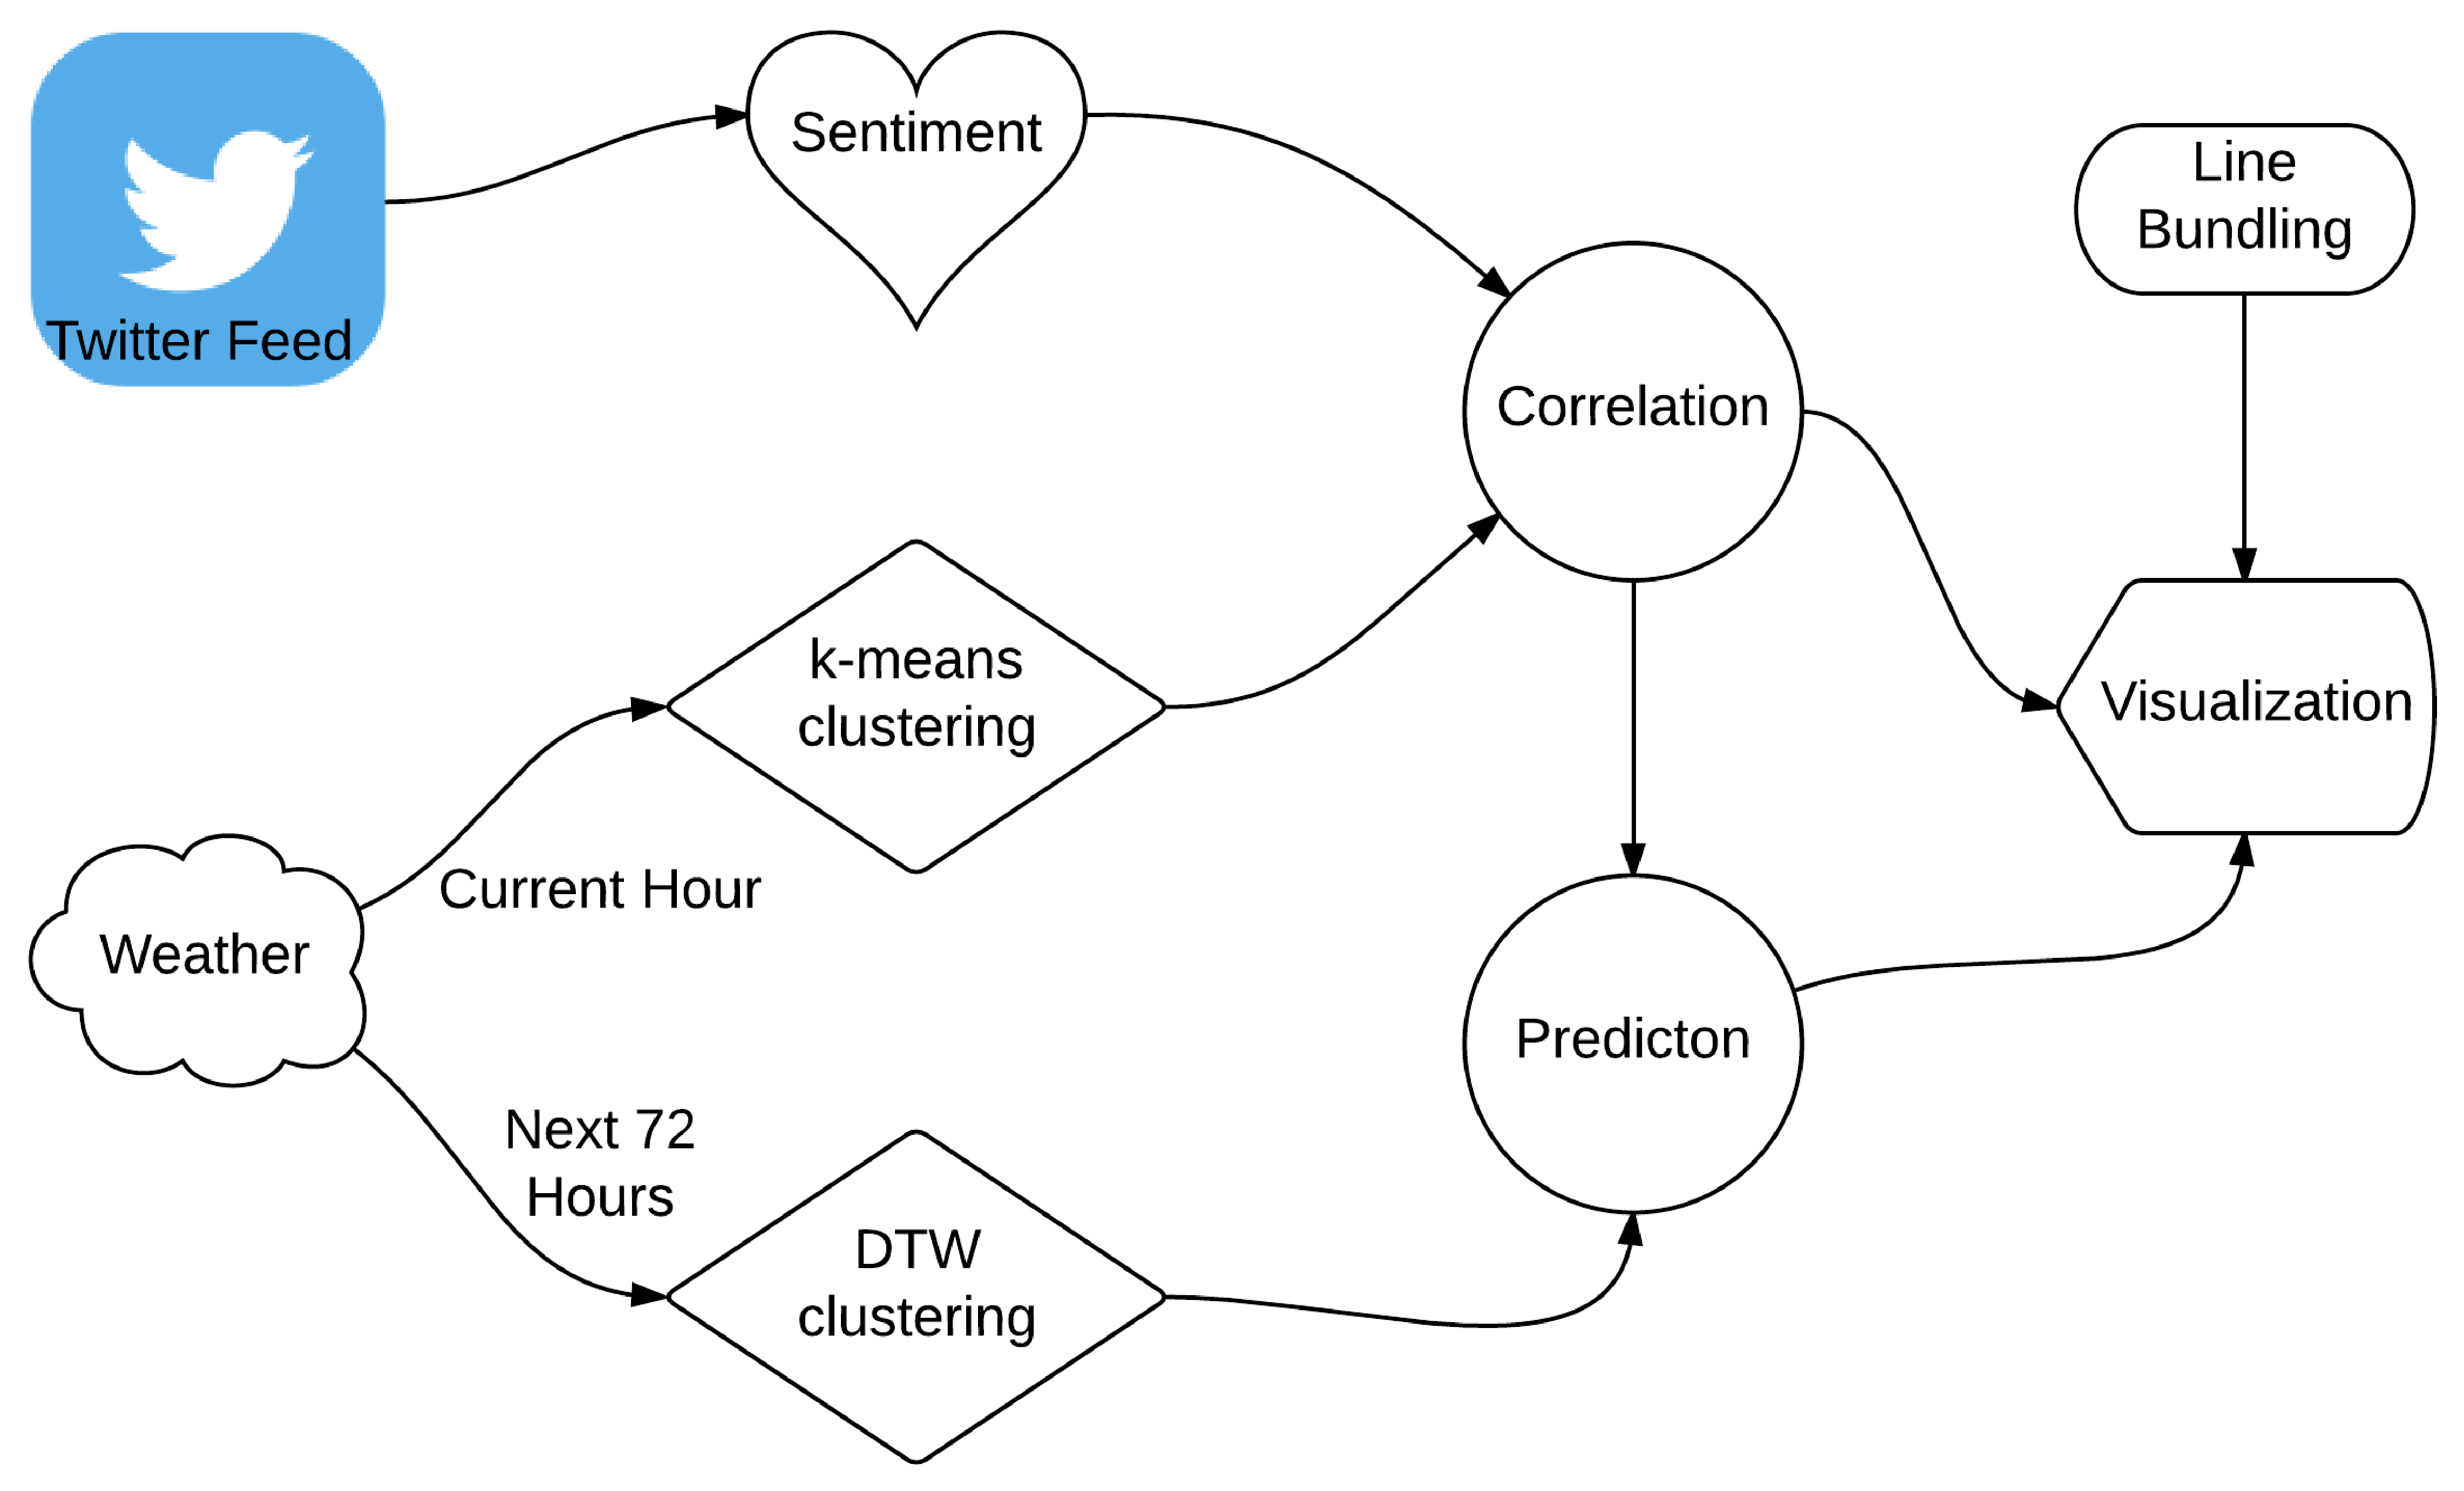
\includegraphics[scale=0.1]{steps}
 \caption{The major steps of Tweether}
 \label{fig:steps}
\end{figure}
%----------------------------------------------------------

\subsection{Data Sets}
\label{sec:dataset}

We use two main data sets with respect to weather and Twitter in this work. The weather data set is generated from a climate simulation using Weather Research and Forecasting (WRF) Model~\cite{Michalakes2004}. %from the Holland Computing Center (HCC).
The data provides hourly forecasts with up to 72 hours in the future. Each WRF file contains multiple variables in regards to weather (i.e., temperature, precipitation, wind speed, etc.). For this visualization, we choose to focus on the surface skin temperature (TSK) variable. Each TSK file is represented via a 2D array %$34 \times 24$
covering a regular geographic region. In this work, we use the WRF data that geographically corresponds to the state of Nebraska.
%The WRF file geographically corresponds to Nebraska and surrounding states as seen in Figure \ref{fig:maps}.

The Twitter data set contains the live data feed from Twitter users throughout Nebraska and is synchronized with the weather data. Only users that have opted-in to turn on the feature of Tweeting With Location are selected. In addition, because Nebraska has a fairly low population with most of the land being barren, only the most populous cities are chosen. These cities include Omaha, Lincoln, Grand Island, Kearney, Fremont, North Platte, Norfolk, Columbus, and Scottsbluff. We use a geographic filtering process to select these cities. The Twitter data is stored in JSON format where we need to extract the coordinates of each tweet and the tweet itself. Due to some cities being on the border of Nebraska such as Omaha, the Twitter data needs to have a second filter which removes any tweets that do not have any relation with Nebraska.

%----------------------------------------------------------
%\begin{figure}[htp]
%  \centering
%  \subfigure[Map showing surrounding states with counties]{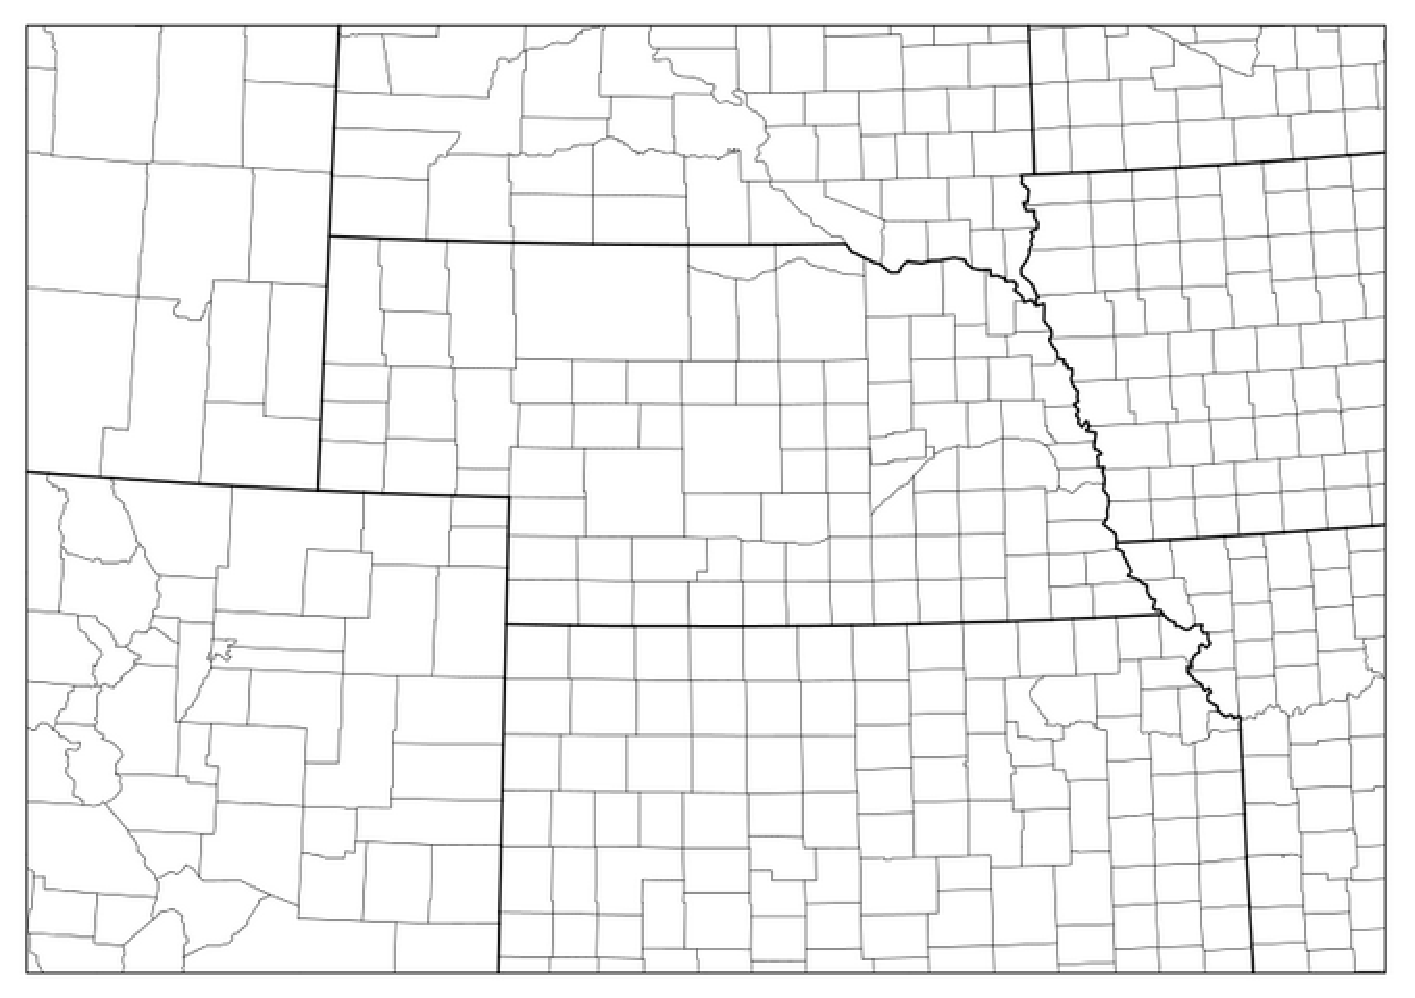
\includegraphics[scale=0.17]{mapBefore}}\quad
%  \subfigure[Map reduced to show prominance to Nebraska]{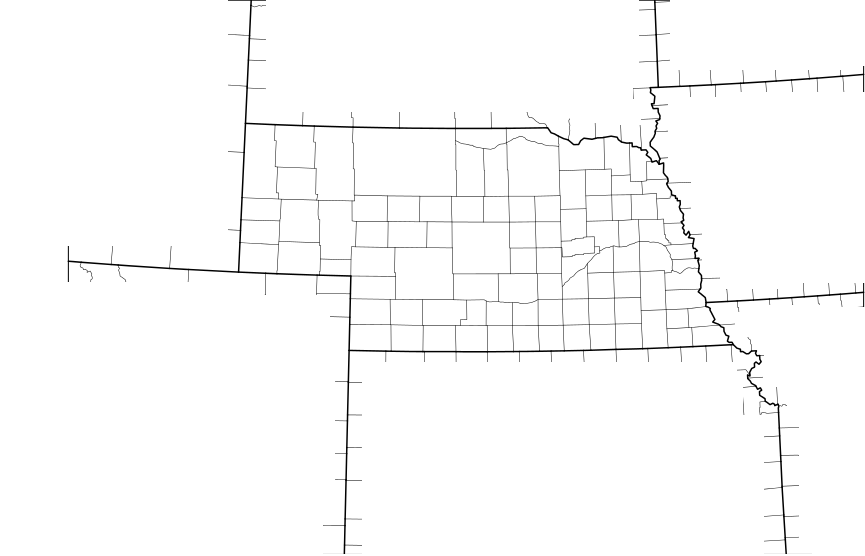
\includegraphics[scale=0.14]{mapAfter}}
%\caption{Nebraska map before and after}
%\label{fig:maps}
%\end{figure}
%----------------------------------------------------------

\subsection{Weather Clustering}
\label{sec:clust}

We use clustering to extract different weather patterns from the WRF data and identify their geographic coverage. The clustering of weather differs depending on if looking at the current hour or the predicted values for the next 72 hours. For the current hour of weather, we use the k-means clustering algorithm. %Since we don't need to worry about the future at the current state nothing additional is added to the algorithm.
For the forecasted weather, we use the dynamic time warping (DTW) algorithm~\cite{salvador2007toward}.

We use the k-means clustering algorithm to partition the 2D array of each time step of TSK into a set of clusters. Some clusters can be dispersed, resulting in random patterns or outliers. These outliers are removed because we assume that moods are affected mostly by comparably dominated weather patterns, and the outliers are small in space and can be changed dynamically in time. To remove outliers, we use a filtering process based on the number of data points in each cluster. If there exists a cluster which has less than one percent of the overall number of clustered elements, this cluster is removed and the data points which belong to a cluster are clustered again. This process is continued until there is no cluster which has less than one percent of the overall cluster count. %In this study, we choose five clusters that gives us good results.
%
For the forecasted weather, we used DTW to measure the similarity between two successive hours, because k-means is not very robust towards outliers due to adding a square weight on the value. 

To smooth any randomness in the cluster values of the 2D array, we use a low-pass filter where the cluster value of an element is determined by the values of surrounding elements.
%connectivity is used to determine the percentage of surrounding elements with the same cluster value as the central element. 
If at least 5 out of 8 neighbors have the same value, the cluster values of the element is kept; otherwise, the value is removed. We found that repeating this operation 4 times to ensure smooth clusters can give use sufficient smooth outcome amongst the majority of 72 hours.
%The number of times to be repeated is chosen due to it creating the most smooth outcome amongst the majority of 72 hours. Figure~\ref{fig:clustering} (d) shows the result of forecasted weather.
Figure~\ref{fig:clustering} (a) shows the distribution of TSK at a certain time step. A directly use of k-means can generate many dispersed small regions, as shown in Figure~\ref{fig:clustering} (b). Our method can clearly extract the dominated TSK patterns, as shown in Figure~\ref{fig:clustering} (c). Figure~\ref{fig:clustering} (d) shows the result of forecasted weather.

%------------------------------------------------
\begin{figure}[t]
\begin{center}
$\begin{array}{c@{\hspace{0.01\linewidth}}c}
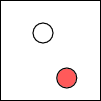
\includegraphics[width=0.45\linewidth]{sample} &
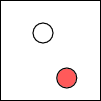
\includegraphics[width=0.45\linewidth]{sample}
\\
\mbox{\small{(a)}} & \mbox{\small{(b)}}
\\
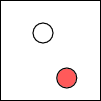
\includegraphics[width=0.45\linewidth]{sample} &
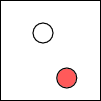
\includegraphics[width=0.45\linewidth]{sample}
\\
\mbox{\small{(c)}} & \mbox{\small{(d)}}
\end{array}$
\end{center}
\vspace{-.1in}
\caption{(a) The distribution of TSK variable at a time step. (b) The k-means result with outliers. (c) The comparably dominated weather patterns. (d) The clustering result of forecasted weather using DTW. }
\label{fig:clustering}
\end{figure}
%------------------------------------------------

\subsection{Sentiment Classification}
\label{sec:senti}

Each tweet can contain different attributes other than plain sentences. Due to each tweet being limited to 140 characters, the majority of users tend to use abbreviations, neologisms (e.g., noob, troll), acronyms hashtags, emoticons, or URL's. Abbreviations, acronyms, and neologisms are taken into account for training our classifier. However, a few items are filtered from certain tweets. The filtering process removes emoticons, URL's, usernames, and hashtags. In some situations, it is known that hashtags can provide instant insight as to what the users are feeling~\cite{keller2005warm}. However, most hashtags that we encountered contain less meaning text or sentences for tags instead of keywords.

We use a \pin{Bayes classifier}~\cite{keller2005warm}\marginnote{\pin{check reference}} to determine the sentiment of tweets. Robert Plutchik's theory~\cite{Plutchik2002} states that there are eight basic emotions:
%----------------------------------------------------------
\begin{itemize}
\vspace{-0.05in}
\setlength{\topsep}{-0.1in}
\setlength{\itemsep}{-0.05in}
\item negative - fear, anger, sadness, depression, disgust
\item positive - joy, trust, anticipation, surprise
\end{itemize}
\vspace{-0.05in}
%----------------------------------------------------------
These emotions are the basic training portion of the classification of tweets. The synonyms for each category are taken into account and this sets up the basic foundation for the tweet classifier.

Other than acronyms we also need to take into account profanity. The use of profanity in social media is very high and it may lead to a positive or negative emotion depending on the situation. To take into account how profanity is used in sentences, we fetched tweets to explore the usage of these words. We found that using these tweets to train the classifier gave a high accuracy rate in regards to profanity. In the beginning, we tried to remove any tweet with profanity, which however drastically lowered our tweet count. We then tried to remove the occurrences of profanity in the tweet and used the remaining words as a judge of emotion, which however only worked in a few cases. For the majority of these tweets, we believed that profanity gave insight to negative moods, and thus decided to take into account profanity.

Due to tweets using abbreviations and incomplete sentences, sentiment calculation is a non-trivial task. The classifier is trained using around 10,000 tweets, where each tweet was given a positive and negative score, and there were rare occurrences of duplicate tweet, and it was made sure that there was an equal portion of positive and negative tweets in regards to words where sentiment could go either way. Figure~\ref{fig:sentiment} shows the sentiment classification results of two time steps.

%------------------------------------------------
\begin{figure}[t]
\begin{center}
$\begin{array}{c@{\hspace{0.01\linewidth}}c}
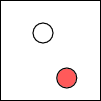
\includegraphics[width=0.45\linewidth]{sample} &
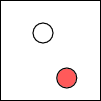
\includegraphics[width=0.45\linewidth]{sample}
\\
\mbox{\small{(a)}} & \mbox{\small{(b)}}
\end{array}$
\end{center}
\vspace{-.1in}
\caption{The sentiment classification results of two time steps }
\label{fig:sentiment}
\end{figure}
%------------------------------------------------


\subsection{Correlation}
\label{sec:corr}

We investigate the correlation between the patterns generated from the weather clustering and the sentiment classification. These patterns are characterized with geographic distributions. Figure~\ref{fig:correlation} (left image) illustrates an examples of two tweets, $T_1$ and $T_2$, and four weather clusters, $W_1$, $W_2$, $W_3$ and $W_4$. It is intuitive that the sentiment derived from a tweet is mostly affected by its overlapped weather cluster. We call such a cluster as the \emph{primary} cluster of a tweet. If there is a naturally geographic overlap between a tweet and a weather cluster, the mapping is pure, as $T_1$ and $W_1$ in Figure~\ref{fig:correlation}. In situations where there is no direct overlap for a tweet to any of the weather clusters the nearest cluster is used, as $T_2$ and $W_1$.

%The correlation between each tweet and the cluster above is represented by a one to one mapping. As we see in Figure \ref{fig:clusters}(a), if there is a natural link then the mapping is pure. In situations where there isn't a direct link to any of the weather clusters the nearest cluster is used.

Other than the natural link between the primary cluster and the tweet, we explore the similarity of connections to other clusters. % regardless of the sentiment it may correspond to.
This is because the sentiment of a tweet can be also affected by its vicinal weather clusters. Therefore, disregarding the primary cluster, we quantify the correlation of the tweet to the other clusters to indicate what other clusters the tweet could map to. In particular, we use the location of a tweet and the TSK value at the location to determine the correlation value to the points of other clusters using the Pearson product-moment correlation coefficient: we determine the similarity of each tweet to the weather clusters:
 %------------------------------------------------
\begin{equation}
\label{eq:pearson}
\rho_{X,Y}=\frac{cov(X,Y)}{\sigma_{X}\sigma_{Y}},
\end{equation}
%------------------------------------------------
where $cov$ is the covariance, and $\sigma_{X}$ ($\sigma_{Y}$) is the standard deviation of $X$ ($Y$). \pin{Here, $X$ and $Y$ are ...} The correlation value of $\rho_{X,Y}$ ranges from -1 to 1. If the value is 1 (-1), it indicates a perfect positive (negative) linear relationship between $X$ and $Y$. If the value is 0, it means that there is no linear relationship between $X$ and $Y$.





In most cases, the secondary and tertiary mapping have the same sentiment since the best fit is a cluster close by with a similar temperature.





This correlation is only available for the current hour. For each tweet, we use the top two relations to other clusters which we deem the \emph{secondary} and \emph{tertiary} clusters, respectively. 
%\marginnote{\pin{why?}}\pin{With a correlation value closer to 1 we keep the sentiment expressed in the primary cluster. However, in the case of a correlation value closer to -1, we swap the sentiment expressed in the primary cluster. We look for the values closest to 1 or -1, and assign the proper sentiment value according to the sign.}


Figure~\ref{fig:correlation} shows the primary, secondary and tertiary clusters of $T_1$ and $T_2$ respectively.

%------------------------------------------------
\begin{figure}[t]
\begin{center}
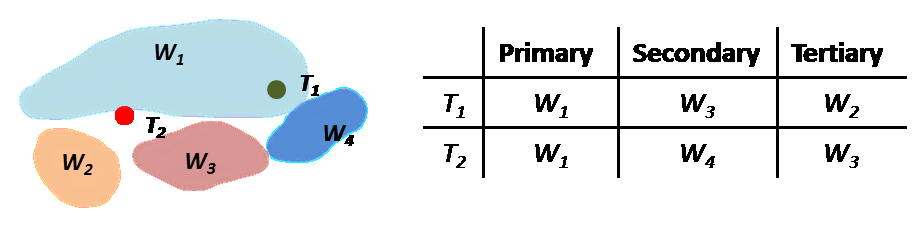
\includegraphics[width=0.9\linewidth]{correlation}
\end{center}
\vspace{-.1in}
\caption{The correlation between the tweets, $T_1$ and $T_2$, and the weather clusters, $W_1$, $W_2$, $W_3$ and $W_4$. The left image shows the geographic distribution of the tweets and the weather clusters. The right table shows the primary, secondary, and tertiary weather clusters of $T_1$ and $T_2$.}
\label{fig:correlation}
\end{figure}
%------------------------------------------------

%%------------------------------------------------
%\begin{figure}[htp]
%  \centering
%  \subfigure[Primary Cluster]{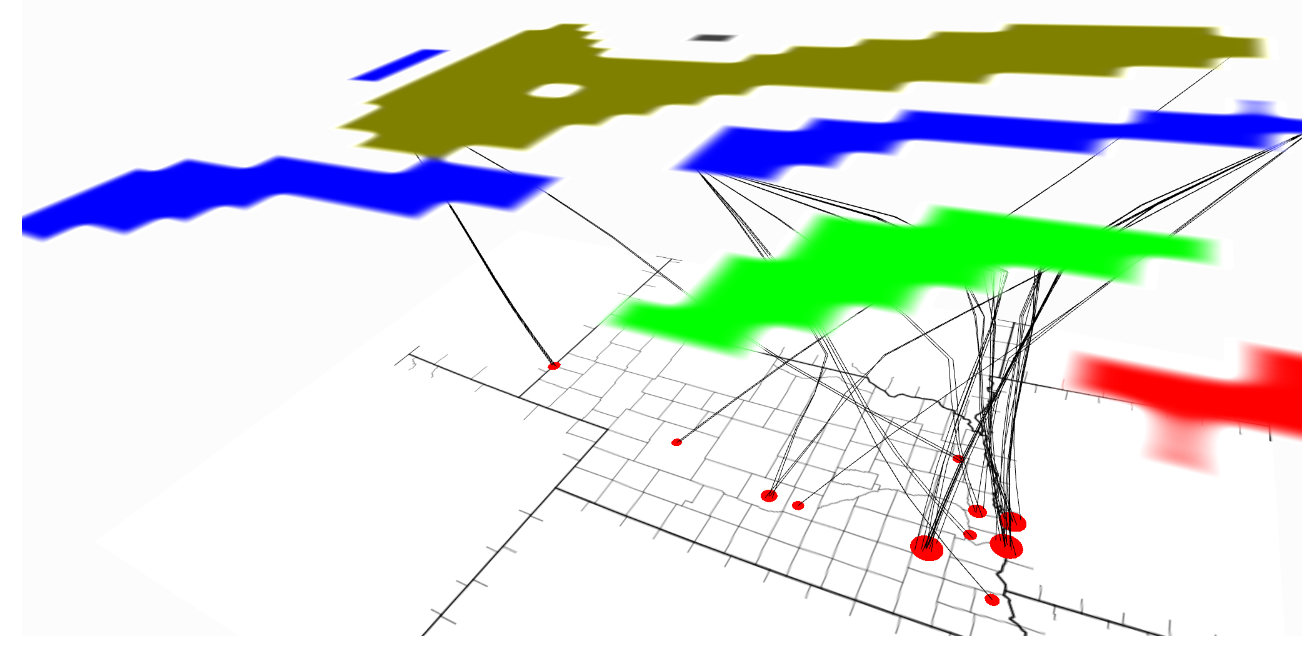
\includegraphics[scale=0.09]{blurBefore}}\quad
%  \subfigure[Secondary Cluster]{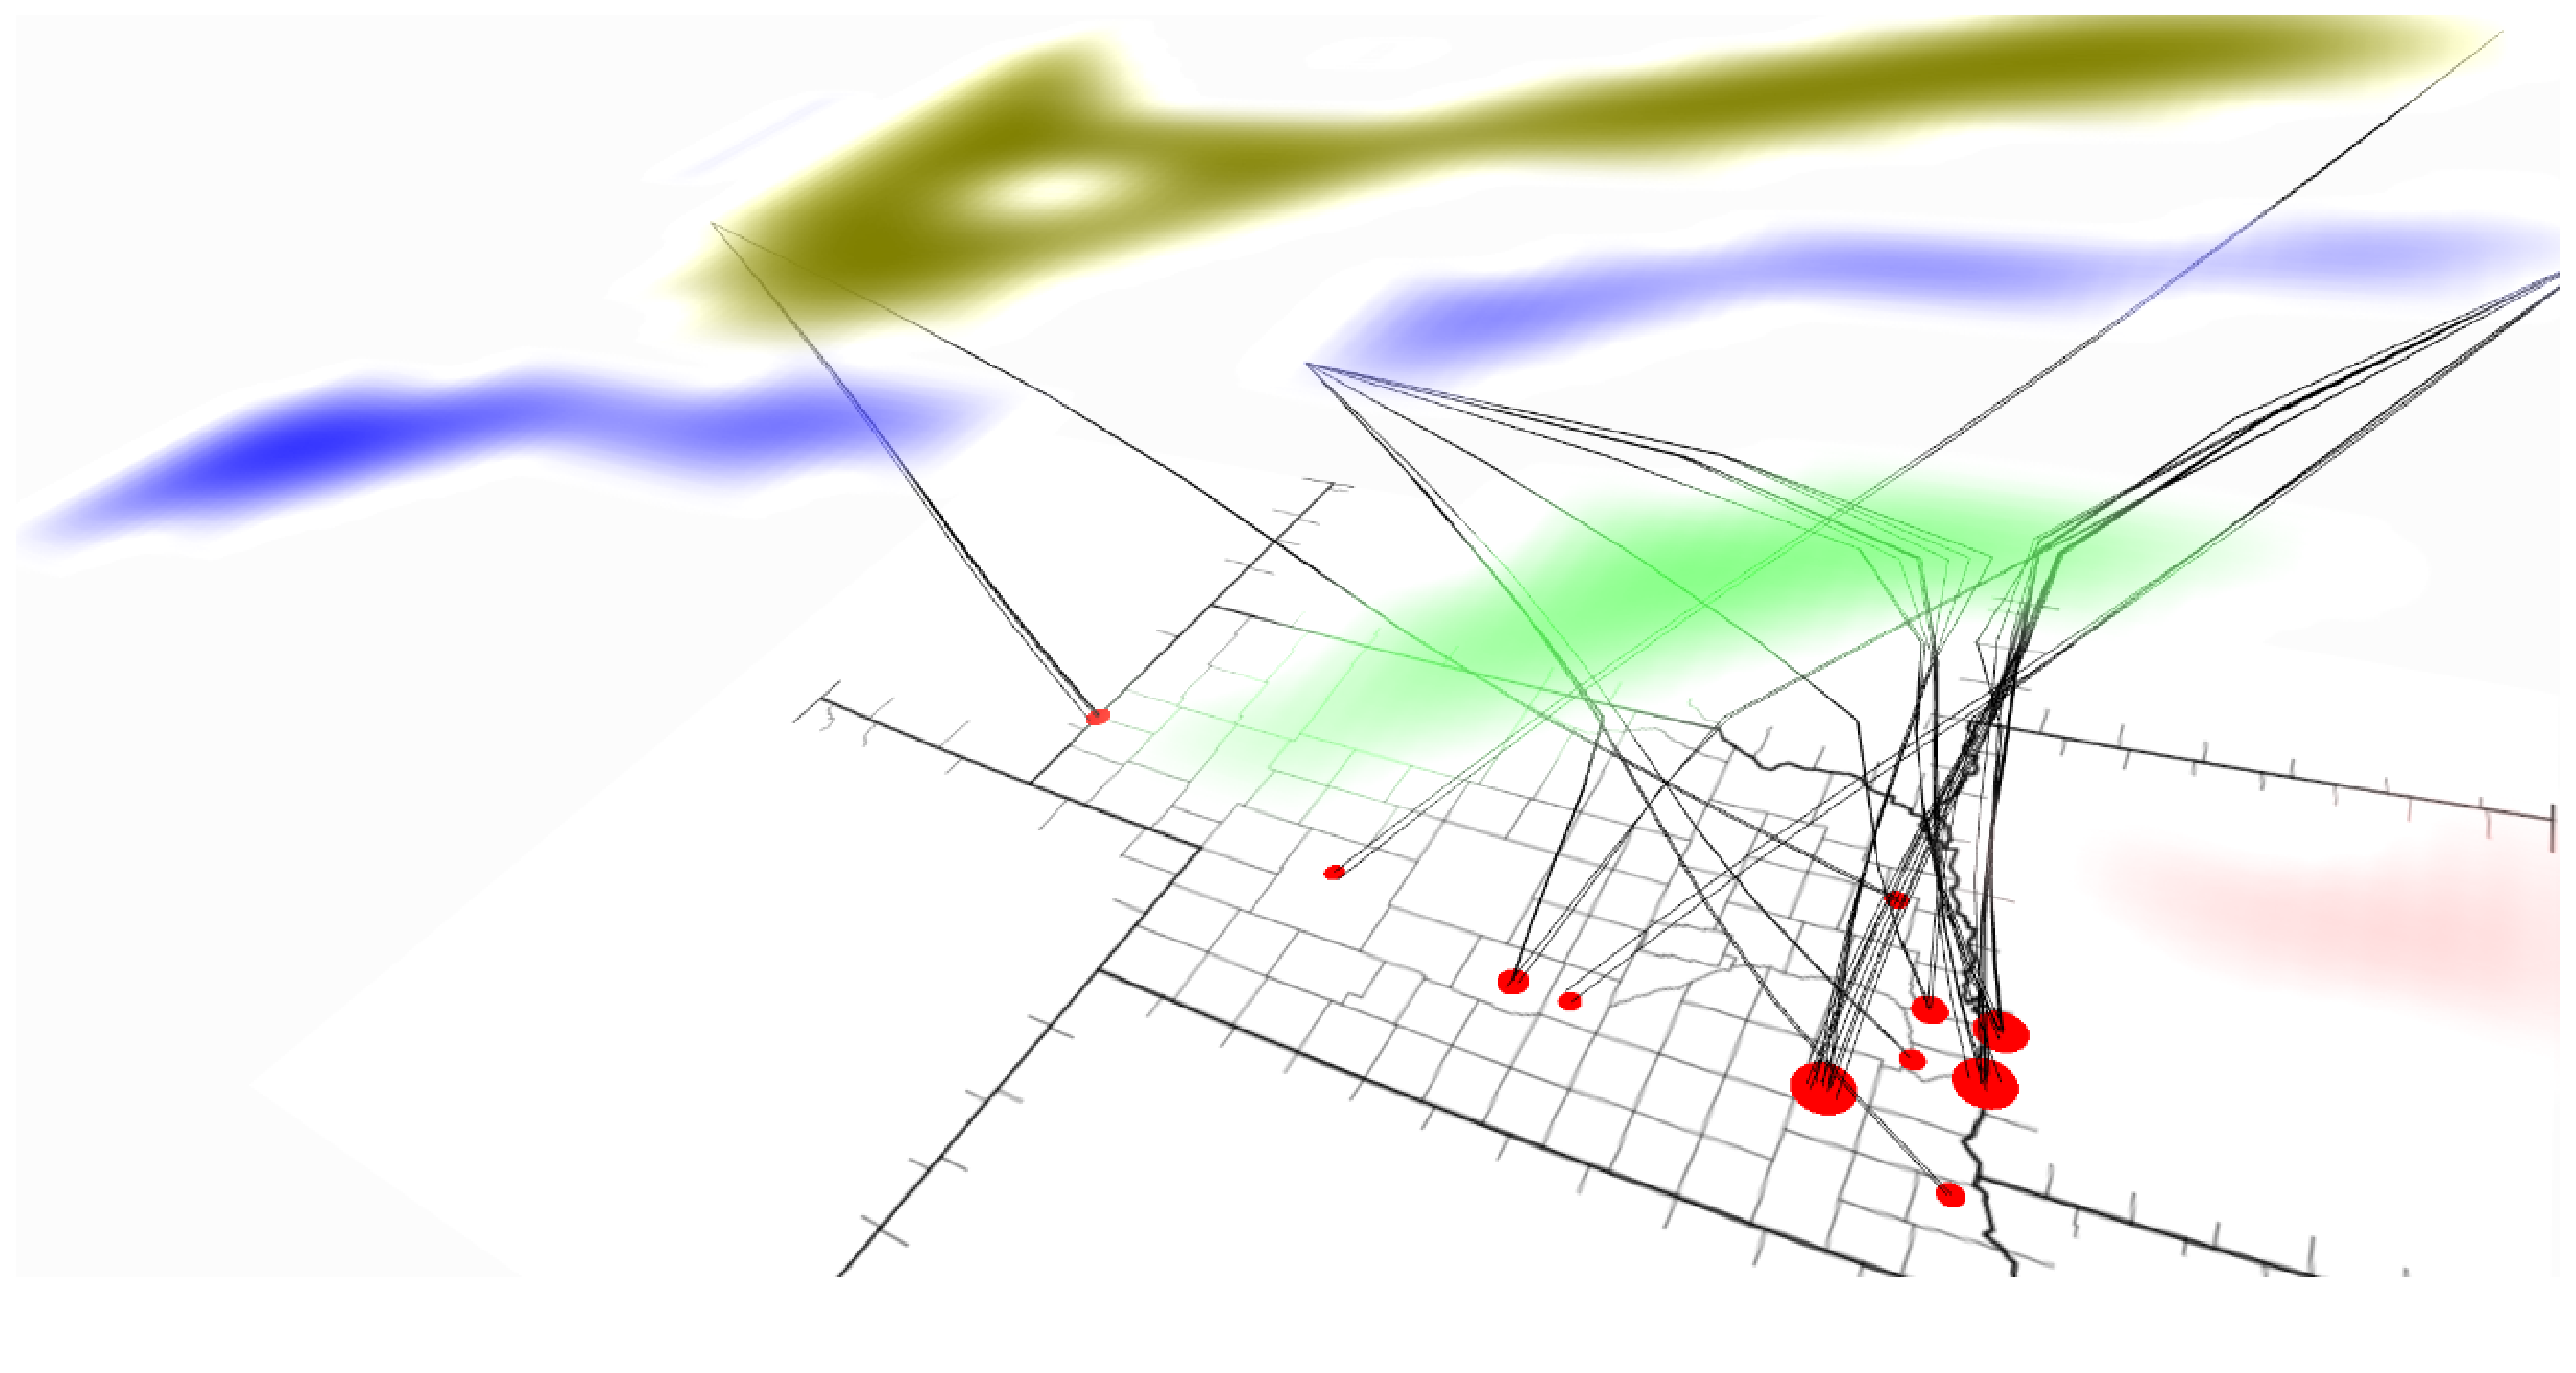
\includegraphics[scale=0.09]{blurAfter}}\quad
%  \subfigure[Tertiary Cluster]{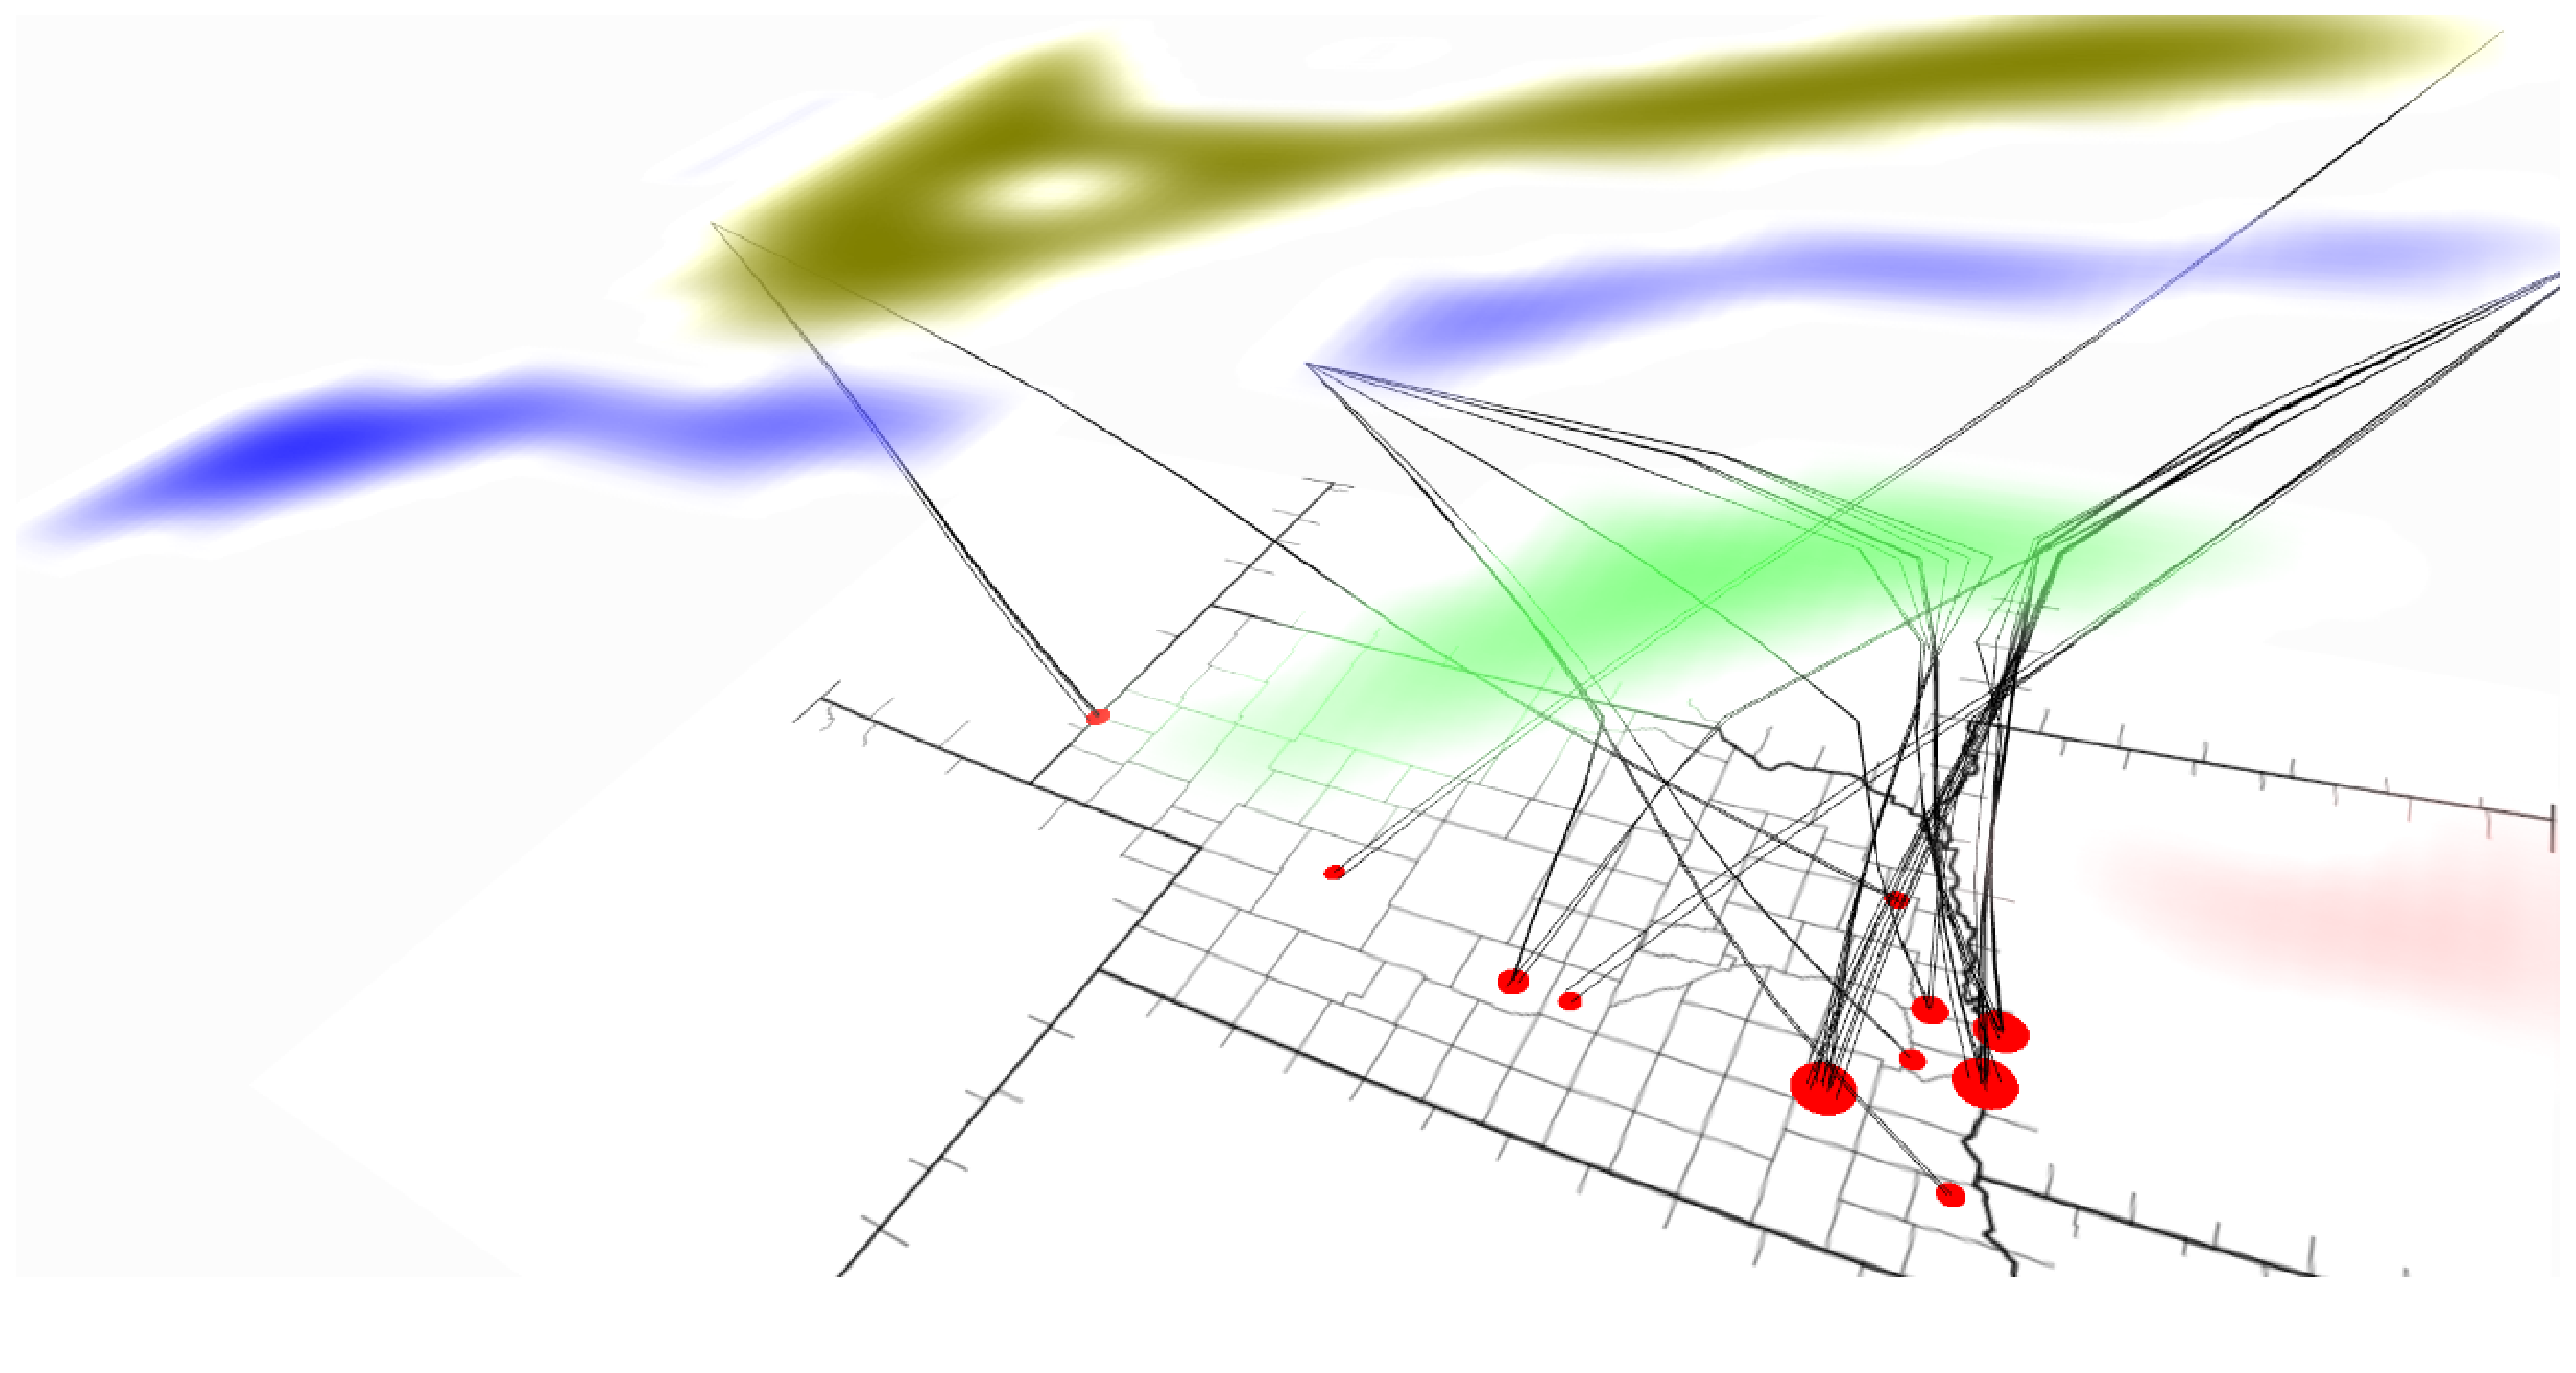
\includegraphics[scale=0.09]{blurAfter}}
%\caption{Clustering of the weather. In this hour, we see five different clusters. The blue cluster is seen in three different locations.}
%\label{fig:clusters}
%\end{figure}
%%------------------------------------------------

%\subsection{Line Bundling}
%\label{sec:line}
%
%We adopt FDEB~\cite{holten2009force} to visualize the graph of correlation. We bundle the related edges with high compatibilities, and iteratively subdivide the edges to generate smooth curves with coherent shapes. This approach can effectively reduce visual clutter in 3D.
%
%The original paper of FDEB~\cite{holten2009force} proposed four criteria, angle, scale, position, and visibility, for edge compatibility measures. In our design, as the edges are mostly oriented along the vertical direction between cloud and ground, the variation in angle or scale is relatively marginal compared to a general graph. In addition, as we display the edges in 3D, the visibility of an edge can be changed from different views. Therefore, only position (i.e., distance between midpoints of edges) is considered for computing edge compatibility in our design.
%
%Similar to FDEB, we use an iterative simulation to refine the bundling. The simulation starts with $P_0$ subdivision points for each edge, and then performs $C$ simulation cycles. During each cycle, a specific number of iteration steps $I$ is conducted to move the subdivision points to reach an equilibrium between forces. The number of iteration steps during the first cycle is $I_0$. After performing a cycle, the number of subdivision points is doubled to smoothen the edges, and the number of iteration steps $I$ is decreased by a factor $R$. We found that a configuration of $P_0=1$, $C=6$, $I_0=50$, and $R=\frac{2}{3}$ leads to appropriate results in our design.


\subsection{Prediction}
\label{sec:pred}

Predicting the future is mostly based on facts. We have at our disposal the current mood and the current temperature, all of the previous days tweets and the temperatures for each hour, and the predicted temperature for each hour for the next two days. Using these facts, we try to determine what the sentiment at each location which people are currently tweeting from will be for the next two days.

Determining the mood of the current locations up to 72 hours in the future is a non-trivial task. Our prediction technique is based on the current hour and the previous day. We choose not to use data from earlier times because the trends today are definitely not the same a year ago, let alone a month ago. In addition to this, we should state that the long-term weather is relatively unpredictable for the state of Nebraska.

%We start with the most rudimentary implementation, by solely comparing which number is closer by simply comparing the difference.
We start with a simple strategy by comparing the temperature difference. If the current temperature is closer to the predicted temperature, we use the sentiment for the current hour to show the prediction. If the sentiment of the hour we are trying to pick has a closer temperature to the same hour of the previous day, we use the sentiment from the previous day.

%Seeing that the previously stated implementation was very crude, we tried a different method.
\pin{However, this simple strategy cannot...}.
Depending on the hour we are trying to predict, we state that if the current hour is at most five hours ago we will place a higher weight on using the current hours values, however when going past five hours we place more weight on the previous days values, where the further we are from the current hour the less weight it plays. Using this method we take the sentiment based on the percentage of the weight.

\pin{The final method we use is a combination of above methods. We first determine the closest temperature value to the hour we are trying to predict the sentiment. Then, based on the difference, we determine the weight the two different sentiment sets place \eqref{eq:w}. As we see in \eqref{eq:p} X and Y represent the current temperature and the previous day's temperature respectively, and Z represents the temperature of the hour that we are trying to predict. The number of good and bad sentiment lines is calculated in \eqref{eq:gb}, where $G$ and $B$ represent the number good and bad tweets predicted by using the good and bad tweets of X and Y. The details regarding how well the different methods performed will be seen later on in the case studies.}

$p_1$ and $p_2$ represent the difference between the temperatures
\begin{equation} \label{eq:p} p_{1}=\left | Z-X \right |	\qquad p_{2}=\left | Z-Y \right |	 \end{equation}

$w_1$ and $w_2$ represent weight of the temperatures
\begin{equation} \label{eq:w} w_{1}=\frac{p_{2}}{p_{1}+p_{2}} 	\qquad w_{2}=\frac{p_{1}}{p_{1}+p_{2}}   \end{equation}

$g_x, g_y, b_x,$ and $b_y$ represent the amount of good and bad tweets in X and Y
\begin{equation} \label{eq:gb}  G = g_{x}w_{1} + g_{y}w_{2}	\qquad B = b_{x}w_{1} + b_{y}w_{2}	 \end{equation}


